\section{混合高斯噪声层}

通常情况下,为了增加策略的稳健性,会对演员网络输出的动作向量添加一个均值为0,标准差为定值的高斯噪声。得到的动作常常还要进行裁剪以防止出现不合理的动作。然而,此种方法需要对两个超参数进行调节,需要大量的时间来进行训练,寻找最优的超参数值。由于在此主体实验中,往往需要训练很长的时间,因此引入这两个超参数并不理想。
    
为了避免手动调节噪声大小,本文提出了一个嵌入演员网络的可自动调节的混合高斯噪声。这个自动调节的噪声向量是通过直接在正态噪声向量后添加全连接层来得到的。得到的噪声向量被加到演员网络最后一层的输出上。
形式化地,给定一个从正态分布中随机采样的$B\times \mathrm{dim}(a)$的高斯噪声矩阵$X_{B\times \mathrm{dim}(a)}$,其中$B$是训练的迁移批次大小,$\mathrm{dim}(a)$是动作空间的维度大小。
如果把演员网络中确定性的部分的输出表示为$f(s)$,其中$s$是输入的状态向量,则有如下缩放后的噪声:

    $$ \mu(s) = f(s) + W X + b, X_{ij}\sim\mathcal N(0,1),$$

    其中$W$和$b$是全连接层的权重,它们通过反向传播自动调节。

    为了更好地展示添加此混合高斯噪声层的效果,研究中在Pyrobolearn中的自定义环境中进行了两个实验以进行对照。其中一个有着固定的噪声大小作为超参数,而另一个没有此超参数而是换成了本文提出的混合高斯噪声层。
    实验系统的基本设计已经在\ref{myenvexp}中进行了详细讨论。本实验中使用了\ref{td3sec}中描述的未来替换方法,与\ref{myenvexp}中不同的是,在这两个实验中对每个网络都多添加了一层隐藏层。此外,随机初始化时对蓝色方块使用了$x,y\in[-1,1]$的均匀采样,WAM机械臂的最后一个末端执行器与方块的距离达到0.5米以内即可获得0.0的奖励,其余情况获得-1.0的奖励,且对靶网络的更新每2个片段进行一次。使用的实验参数如表\ref{fcntable}所示,其中符号的意义与\ref{pretable}中相同。

    \begin{table}[htbp]
        \caption{混合高斯噪声层实验参数}
        \label{fcntable}
    \vspace{0.5em}\centering\wuhao
    \begin{tabular}{ccccc}
    \toprule[1.5pt]
    实验参数 & 值\\
    \midrule[1pt]
        $\epsilon_{noise}$ & 0.2\\
        $\sigma_{clip}$ & 0.5\\
        $M$ & $5\times 10^3$\\
        $\epsilon_{rand}$ & 0.3\\
        $\gamma$ & 0.991\\
        $\alpha$ & $3\times 10^{-4}$\\
        $B$ & 16\\
        $\tau$ & 0.005\\
        $T$ & 50\\
        $f_\mu$ & 2\\
        $T_{start}$ & $2.5\times 10^4$\\
        $N_{sample}$ & 200 \\
        $k$ & 18\\
        $K_{replay}$ & 4\\
        $\xi_{LSH}$ & $2\times 10^{-2}$\\
    \bottomrule[1.5pt]
    \end{tabular}
    \end{table}
    其中$k$是\ref{LSHsec}中的超参数,用于调整对状态空间离散化的粒度。
    $K_{replay}$是\ref{HERsec}中所述的超参数,它与替换掉的迁移的比例有关。
    $\xi_{LSH}$是在计算最终奖励时,基于局部敏感哈希和计数的探索奖励的系数。
    其余参数的意义与表\ref{pretable}中相同。

    平均每个片段的使用混合高斯噪声层的演员网络的损失和使用噪声大小超参数的演员网络的损失如图\ref{fcn_lossmu}所示。有混合高斯噪声层的演员网络的损失在较少的代数内上升到了一个相对较低的值。由于这两组实验中损失都收敛到了较高的值,此损失曲线并不能明确反映哪种方法更优,因为演员网络的损失是由评论家网络决定的,而这两组实验中的评论家并不一定具有相同权重,因此即使是相同的演员网络也有可能具有不同的损失。

        \begin{figure}[htpb]
        \centering
        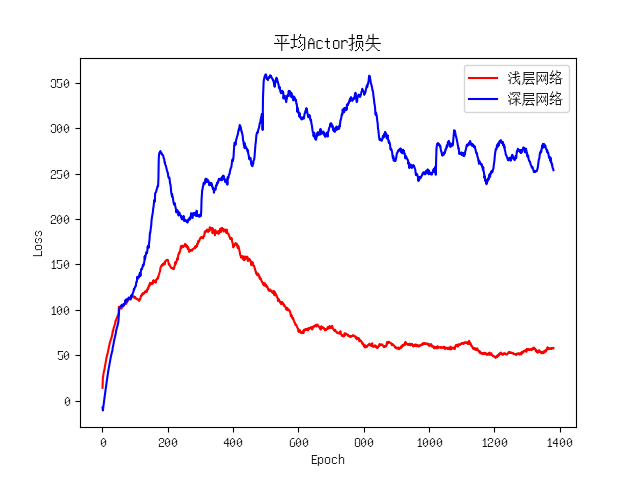
\includegraphics[width=0.6\textwidth]{myenv_lossmu.png}
        \caption{演员网络$\mu$的损失曲线}
            \label{fcn_lossmu}
        \end{figure}

    每个片段的评论家网络$Q_1$和$Q_2$的平均损失分别如图\ref{fcn_lossq1}和图\ref{fcn_lossq2}所示。可以看出,它们的损失也是和演员网络$\mu$的损失具有相似的形状。由于评论家网络的损失也并没有收敛到较低的值,这些损失曲线也不能反映混合高斯噪声层带来的变化。但是可以肯定的是,添加混合高斯噪声层后损失曲线变化更加平缓了。从图中也可以看出,评论家网络的损失比演员网络的损失更加不稳定,这可能是由于评论家网络的损失直接与环境相关导致的。

        \begin{figure}[htpb]
        \centering
        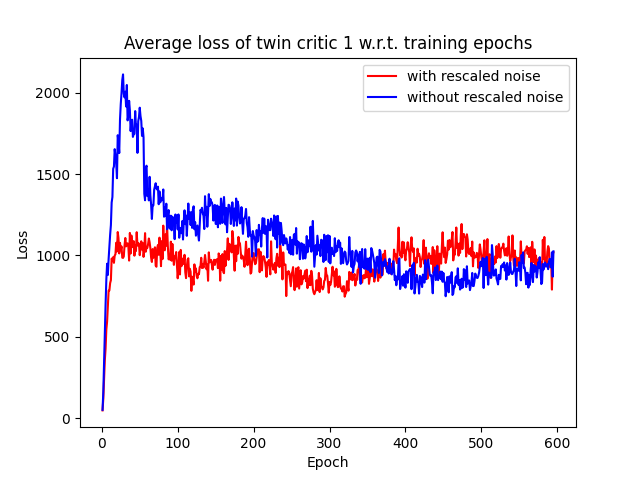
\includegraphics[width=0.6\textwidth]{myenv_lossq1.png}
        \caption{评论家网络$Q_1$的损失曲线}
            \label{fcn_lossq1}
        \end{figure}

        \begin{figure}[htpb]
        \centering
        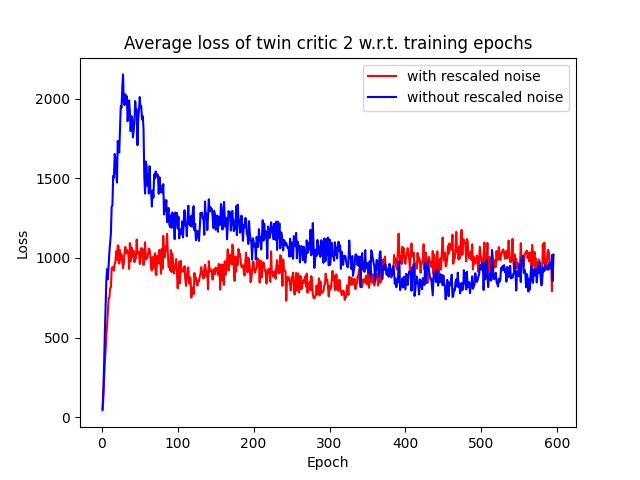
\includegraphics[width=0.6\textwidth]{myenv_lossq2.png}
        \caption{评论家网络$Q_2$的损失曲线}
            \label{fcn_lossq2}
        \end{figure}

        使用和不使用混合高斯噪声层的单位片段平均环境奖励如图\ref{fcn_reward}所示。可以看出,添加了混合高斯噪声层的方法获得的奖励要稍微比只使用噪声大小超参数的方法更高。

        \begin{figure}[htpb]
        \centering
        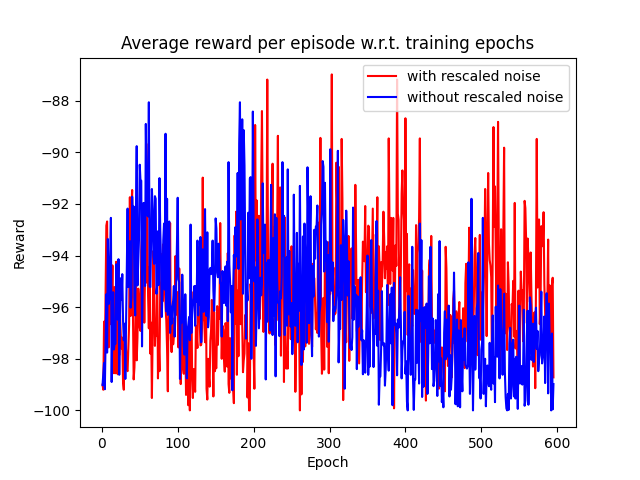
\includegraphics[width=0.6\textwidth]{myenv_reward.png}
        \caption{平均环境奖励曲线}
            \label{fcn_reward}
        \end{figure}

        平均成功率曲线的变化趋势与平均环境奖励的大致相同。对于最后的平均成功率,添加了混合高斯噪声层的要稍微更高。

        \begin{figure}[htpb]
        \centering
        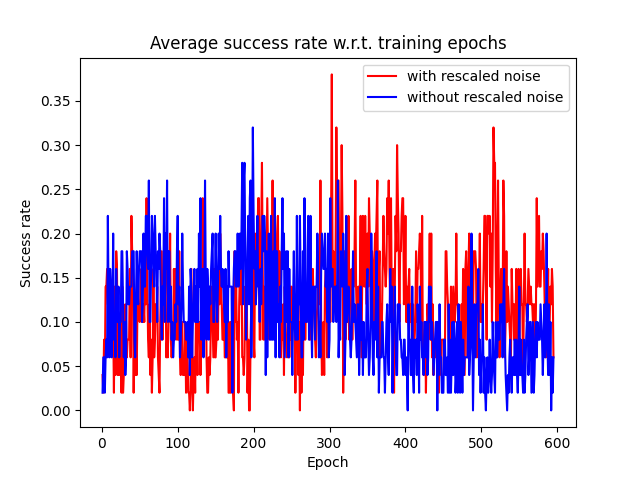
\includegraphics[width=0.6\textwidth]{myenv_suc_rate.png}
        \caption{任务目标成功率}
            \label{fcn_suc_rate}
        \end{figure}

        在引入混合高斯噪声层之后,本研究中使用的TD3算法实际上由确定性策略梯度算法转化为了非确定性策略梯度算法。
        混合高斯噪声层通过自适应地调整噪声向量的大小和方向,可以更好地适应开放任务中复杂的动力学过程,更好地探索低概率的动作,防止策略收敛到局部最优,并加速算法的收敛。

